% =====================================================================
% Overleaf compiler setting: this file has no Korean text, so the
% default pdfLaTeX compiler works fine (no kotex / XeLaTeX needed).
% =====================================================================
\documentclass[conference]{IEEEtran}

\usepackage{amsmath,amssymb}
\usepackage{graphicx}
\usepackage{booktabs}
\usepackage{hyperref}
\usepackage{caption}

\title{Effect of the KL Coefficient on the Reward--Diversity\\Trade-off in PPO-based RLHF Fine-tuning:\\A Case Study on KoChatGPT}

\author{
  \IEEEauthorblockN{Yongseok Oh}
  \IEEEauthorblockA{ysoh1113@gmail.com}
}

\begin{document}
\maketitle

\begin{abstract}
The final stage of Reinforcement Learning from Human Feedback (RLHF),
PPO fine-tuning, is characterized by a trade-off between reward
maximization and a KL penalty that discourages the policy from
drifting too far from the initial policy. The KL coefficient $\beta$,
which controls this trade-off, was left at its untested library
default (0.1) in KoChatGPT (airobotlab, 2023; built on ColossalAI
Coati), a widely used Korean RLHF tutorial project. We perform a
controlled sweep over $\beta \in \{0, 0.02, 0.05, 0.1, 0.3, 1.0\}$,
together with a 2-extra-seed replication for three of these conditions
($\beta{=}0, 0.02, 0.1$), to quantify how $\beta$ affects reward,
empirical KL divergence, and generation diversity in a KoGPT2-based
RLHF-PPO pipeline. Our results show that (i) at this experimental
scale (1--3 seeds per condition, 10 episodes), all six PPO-fine-tuned
conditions achieve a lower mean reward than the SFT baseline; (ii) a
sample-level repetition-rate metric reveals repetition-collapse
tendencies in the baseline as well as nearly every condition,
suggesting that this behavior originates in the SFT stage rather than
being induced by $\beta$; (iii) in the seed-repeat experiment,
differences across $\beta$ within a fixed seed are smaller than
differences across seeds, indicating that at this scale the effect of
$\beta$ can be masked by seed-level variance; and (iv) a corpus-pooled
distinct-n metric can be quantitatively shown to misclassify a
condition with genuine per-sample repetition collapse as sufficiently
diverse, motivating a sample-level repetition-rate metric as a
complementary criterion.
\end{abstract}

% =====================================================================
\section{Introduction}
% =====================================================================

RLHF consists of three stages: (i) supervised fine-tuning (SFT), (ii)
reward model (RM) training, and (iii) PPO-based policy fine-tuning. In
this last stage, the policy is optimized to maximize the reward
model's score while being regularized by a KL divergence term that
keeps it from drifting too far from the original (SFT) policy. Although
the coefficient $\beta$ that controls the strength of this
regularization is a key RLHF hyperparameter, open-source tutorial
implementations often leave it at its untested default value.

We extend \textbf{KoChatGPT}~\cite{kochatgpt2023,
colossalchat2023}, a Korean-language tutorial that reproduces an RLHF
pipeline for KoGPT2 using the ColossalAI Coati library. Inspecting the
actual library source code revealed that the KL coefficient argument
(\texttt{kl\_coef}) of \texttt{PPOTrainer} defaults to 0.1, and that
the KoChatGPT tutorial uses this value without ever validating it.
We extend the original tutorial precisely at this point -- by
systematically testing how $\beta$ actually affects the outcome --
through a grid sweep and a multi-seed replication.

\subsection{Research Questions and Hypotheses}
\begin{itemize}
  \item \textbf{H1.} Smaller $\beta$ yields a higher reward-model
        score but lower generation diversity (a reward--diversity
        trade-off).
  \item \textbf{H2.} Larger $\beta$ keeps the policy too close to the
        SFT model, resulting in little reward improvement.
  \item \textbf{H3.} There exists an intermediate $\beta$ that improves
        reward while avoiding severe text collapse.
\end{itemize}

\subsection{Contributions}
\begin{itemize}
  \item We systematically sweep the previously untested KL coefficient
        $\beta$ in the PPO stage of KoChatGPT, and implement the sweep
        in a reproducible manner grounded in the actual library source
        (the reward computation and the KL estimator it uses).
  \item In addition to corpus-pooled distinct-n, we define a
        sample-level repetition-rate metric and a degeneracy criterion
        based on it, integrate them into the model-selection rule, and
        quantitatively show that this metric detects repetition
        collapse that the corpus-level metric alone misses.
  \item We replicate three $\beta$ values with two additional random
        seeds and quantitatively compare the resulting across-$\beta$
        differences against across-seed variance.
\end{itemize}

% =====================================================================
\section{Background}
% =====================================================================

\subsection{PPO-based RLHF}

When fine-tuning an initial policy $\pi_{\text{SFT}}$ (obtained via
SFT) against a reward model $r_\phi(x,y)$, the KL-regularized reward
is defined as~\cite{ziegler2019finetuning, ouyang2022instructgpt}:

\begin{equation}
R(x, y) = r_\phi(x, y) - \beta \cdot D_{\mathrm{KL}}\big(\pi_\theta(\cdot \mid x)
\,\|\, \pi_{\text{SFT}}(\cdot \mid x)\big)
\label{eq:reward}
\end{equation}

The policy $\pi_\theta$ is trained with the clipped PPO objective
\cite{schulman2017ppo}:

\begin{equation}
L^{\mathrm{CLIP}}(\theta) = \mathbb{E}_t\Big[\min\big(\rho_t(\theta)
\hat{A}_t,\ \mathrm{clip}(\rho_t(\theta),\, 1-\epsilon,\, 1+\epsilon)\,
\hat{A}_t\big)\Big]
\label{eq:ppo}
\end{equation}

where $\rho_t(\theta) = \pi_\theta(a_t \mid s_t) / \pi_{\theta_{\text{old}}}(a_t
\mid s_t)$ and $\hat{A}_t$ is the GAE-based advantage estimate.

% =====================================================================
\section{Related Work}
% =====================================================================

\textbf{Base system.} KoChatGPT~\cite{kochatgpt2023}, the tutorial we
extend, reproduces a KoGPT2-based SFT--RM--PPO pipeline using
ColossalAI's Coati (\texttt{applications/Chat})~\cite{colossalchat2023}
library.

\textbf{KL-regularized RLHF.} The objective in
Eq.~\eqref{eq:reward} was first proposed by Ziegler et
al.~\cite{ziegler2019finetuning}; Stiennon et
al.~\cite{stiennon2020learning} established the reward--KL frontier as
a standard way to present such results; and Ouyang et al.
(InstructGPT)~\cite{ouyang2022instructgpt} applied it at large
commercial scale. Our experimental design (grid sweep, reward--KL
frontier plot) follows this lineage directly, and additionally reports
confidence intervals from multi-seed replication in a small-scale
reproduction setting.

\textbf{Reward overoptimization.} Gao et al.~\cite{gao2023scaling}
analyzed, via large-scale scaling laws, the phenomenon in which
over-optimizing against a reward model raises reward scores without
tracking true preferences. The reward model used in our experiments
was trained on only a fraction of the available ranking data and may
therefore be relatively noisy, which is relevant to the interpretation
of results discussed in \S\ref{sec:discussion}.

\textbf{Limitations of diversity metrics.} The distinct-n metric was
proposed by Li et al.~\cite{li2016diversity}; Holtzman et
al.~\cite{holtzman2020curious} pointed out that corpus-level aggregated
metrics can miss degeneration in individual samples. We confirm this
limitation numerically in our experiments (\S\ref{sec:discussion}).

% =====================================================================
\section{Method}
% =====================================================================

\subsection{Base System}

The actor is initialized from the SFT checkpoint, and both the critic
and the reward model are initialized from the RM checkpoint; the
initial model is a frozen reference policy equal to the SFT policy.
\texttt{PPOTrainer}'s default hyperparameters are
\texttt{kl\_coef=0.1}, \texttt{eps\_clip=0.2}, and
\texttt{value\_clip=0.4}. The reward model was trained on only 10\% of
the KoChatGPT tutorial's ranking data (\texttt{total\_using\_ratio=0.1}).

\subsection{Proposed Extension: KL Coefficient Sweep}

To quantify how $\beta$ affects the reward--diversity trade-off, we
independently ran PPO fine-tuning over the grid $\mathcal{B} = \{0,
0.02, 0.05, 0.1, 0.3, 1.0\}$ ($\beta{=}0.1$ corresponds to the
tutorial's untested default). All hyperparameters other than $\beta$,
and the initial checkpoints, were held fixed so that any observed
difference is attributable to $\beta$ alone. For a fair comparison
across conditions, the actor/critic/initial model were re-initialized
from the SFT/RM checkpoints for every value of $\beta$.

\subsection{Seed-Repeat Experiment}
\label{sec:seedrepeat}

A single-seed sweep alone cannot distinguish whether differences
across conditions are a systematic effect of $\beta$ or noise from the
stochasticity of training (rollout sampling, parameter
initialization, etc.). To assess this, we repeated training for three
conditions ($\beta \in \{0, 0.02, 0.1\}$) with two additional random
seeds (\texttt{seed}$\in\{1,2\}$), and combined these with the
original sweep's result (treated as \texttt{seed}$=0$) to compute the
mean and standard deviation over three observations per condition.

\subsection{Evaluation Protocol}

For each condition, we generated with greedy decoding on $N{=}30$
held-out prompts (not used in training) and measured the following.

\begin{itemize}
  \item \textbf{Reward score}: mean/standard deviation of the score
        assigned by $r_\phi$.
  \item \textbf{Empirical KL}: computed using Schulman's low-bias k3
        estimator \cite{schulman2017ppo}.
        \begin{equation}
        \widehat{D}_{\mathrm{KL}} = \mathbb{E}\big[(e^{\Delta} - 1) -
        \Delta\big], \quad \Delta = \log\pi_\theta(a\mid s) -
        \log\pi_{\text{SFT}}(a\mid s)
        \label{eq:klhat}
        \end{equation}
  \item \textbf{Distinct-n}~\cite{li2016diversity}: the unique n-gram
        ratio computed by pooling all 30 held-out generations together.
        \begin{equation}
        \text{distinct-}n = \frac{|\{\text{unique } n\text{-grams}\}|}
        {|\{\text{total } n\text{-grams}\}|}
        \label{eq:distinctn}
        \end{equation}
  \item \textbf{Sample-level repetition rate}: measures the degree of
        repetition within an individual response $y$, capturing
        single-sample collapse that a corpus-level distinct-n can miss.
        \begin{equation}
        \text{rep}(y) = 1 - \frac{|\{\text{unique bigrams in } y\}|}
        {|\{\text{total bigrams in } y\}|}
        \label{eq:reprate}
        \end{equation}
        computed on the generated continuation only (prompt excluded,
        based on the action mask).
  \item \textbf{Degeneracy flag}: a response $y$ is flagged as
        degenerate if its repetition rate exceeds a threshold or if
        the number of generated tokens is too small (i.e., effectively
        empty).
        \begin{equation}
        \text{is\_degenerate}(y) = \mathbb{1}\big[\text{rep}(y) > \tau_{\text{rep}}
        \ \lor\ |y| < \tau_{\text{len}}\big]
        \label{eq:degenerate}
        \end{equation}
        A condition is marked \texttt{any\_degenerate}$=$True if at
        least one of its 30 evaluation responses is flagged.
\end{itemize}

\subsection{Model Selection Criterion}
\label{sec:selection}

The best model is selected as the condition with the highest reward
score among those that (a) retain at least 70\% of the pre-training
(SFT) distinct-2 and (b) have \texttt{any\_degenerate}$=$False.

\begin{equation}
\beta^{*} = \operatorname*{argmax}_{\beta \in \mathcal{B}'} \
\overline{r_\phi}(\beta), \quad
\mathcal{B}' = \{\beta \in \mathcal{B} : \text{distinct2}(\beta) \geq
0.7 \times \text{distinct2}_{\text{SFT}} \ \land \ \lnot\,\text{any\_degenerate}(\beta)\}
\label{eq:selection}
\end{equation}

If $\mathcal{B}'$ is empty, $\beta^{*}$ is reported as undefined
(see \S\ref{sec:results}).

% =====================================================================
\section{Experimental Setup}
% =====================================================================

\begin{table}[h]
\centering
\caption{Fixed hyperparameters}
\label{tab:setup}
\begin{tabular}{@{}ll@{}}
\toprule
Item & Value \\
\midrule
Base model & KoGPT2 (\texttt{skt/kogpt2-base-v2}) \\
PPO data & \texttt{kochatgpt\_3\_PPO.jsonl} \\
RM training data fraction & 10\% (\texttt{total\_using\_ratio=0.1}) \\
$\beta$ grid & $\{0, 0.02, 0.05, 0.1, 0.3, 1.0\}$ \\
$\beta$ values replicated & $\{0, 0.02, 0.1\}$ (2 extra seeds) \\
\texttt{max\_epochs} & 1 \\
\texttt{train\_batch\_size} & 8 \\
\texttt{num\_episodes} & 10 \\
\texttt{max\_timesteps} & 3 \\
\texttt{update\_timesteps} & 3 \\
\texttt{eps\_clip} & 0.2 \\
\texttt{value\_clip} & 0.4 \\
Eval. prompts & 30 (held-out) \\
Eval. decoding & greedy \\
Training decoding & sampling (top-k=50, T=1.0) \\
\bottomrule
\end{tabular}
\end{table}

% =====================================================================
\section{Results}
\label{sec:results}
% =====================================================================

\begin{table}[h]
\centering
\caption{$\beta$ sweep results (single seed per condition, $N{=}30$)}
\label{tab:results}
\small
\begin{tabular}{@{}lccccc@{}}
\toprule
$\beta$ & Reward & KL & D-1 & D-2 & max rep \\
\midrule
baseline (SFT) & 2.545 & 0.000 & 0.683 & 0.762 & 0.950 \\
0.00           & 1.815 & 0.258 & 0.407 & 0.521 & 0.952 \\
0.02           & 1.992 & 0.129 & 0.608 & 0.734 & 0.794 \\
0.05           & 1.780 & 0.115 & 0.652 & 0.764 & 0.950 \\
0.10           & 2.194 & 0.164 & 0.449 & 0.531 & 0.942 \\
0.30           & 2.136 & 0.291 & 0.494 & 0.608 & 0.950 \\
1.00           & 1.589 & 0.109 & 0.495 & 0.634 & 0.800 \\
\bottomrule
\end{tabular}
\end{table}

All seven conditions are flagged \texttt{any\_degenerate}$=$True (i.e.,
at least one of the 30 evaluation responses satisfies the degeneracy
criterion of Eq.~\eqref{eq:degenerate}), so $\mathcal{B}'$ in
Eq.~\eqref{eq:selection} is empty and $\beta^{*}$ is undefined
(\texttt{best\_kl\_coef=None}). All six PPO conditions achieve a lower
mean reward than the SFT baseline (2.545).

\begin{figure}[h]
\centering

\includegraphics[width=\linewidth]{kl_sweep_plots.png}
\caption{Reward--KL frontier (left) and distinct-2 as a function of
$\beta$ (right) across the six conditions. Points are shown without
connecting lines, reflecting as-is that the empirical KL is not
monotonic in the ordering of $\beta$.}
\label{fig:frontier}
\end{figure}

\begin{table}[h]
\centering
\caption{Seed-repeat experiment: mean $\pm$ std. over 3 seeds ($\beta\in\{0,0.02,0.1\}$)}
\label{tab:seedrepeat}
\small
\begin{tabular}{@{}lccc@{}}
\toprule
$\beta$ & Reward & KL & Distinct-2 \\
\midrule
0.00 & $2.038 \pm 0.240$ & $0.326 \pm 0.082$ & $0.624 \pm 0.094$ \\
0.02 & $2.102 \pm 0.179$ & $0.284 \pm 0.145$ & $0.695 \pm 0.045$ \\
0.10 & $2.196 \pm 0.181$ & $0.298 \pm 0.120$ & $0.631 \pm 0.088$ \\
\bottomrule
\end{tabular}
\end{table}

\begin{figure}[h]
\centering
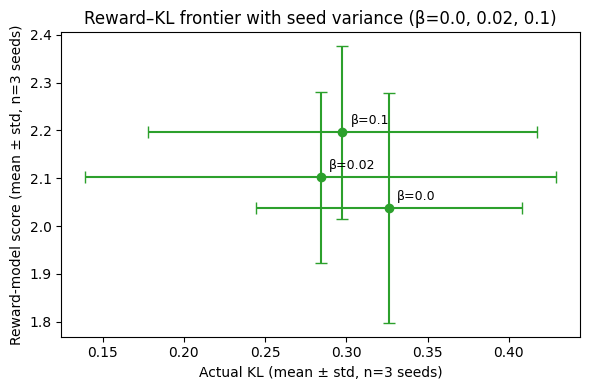
\includegraphics[width=\linewidth]{kl_seed_repeat_plot.png}
\caption{Reward--KL frontier for $\beta \in \{0, 0.02, 0.1\}$ (mean
$\pm$ std., $n{=}3$ seeds). The error bars are as large as or larger
than the differences between condition means, showing that at this
scale the effect of $\beta$ is not clearly distinguishable from
seed-level variance.}
\label{fig:seedrepeat}
\end{figure}

As shown in Table~\ref{tab:seedrepeat} and Fig.~\ref{fig:seedrepeat},
the largest difference in mean reward across $\beta$ is $0.16$
($\beta{=}0.00$ vs.\ $\beta{=}0.10$), whereas the across-seed standard
deviation within each $\beta$ is $0.18$--$0.24$, i.e., as large as or
larger than that. In other words, at this experimental scale, the
average difference obtained by changing $\beta$ is smaller than the
difference obtained by simply re-running the same $\beta$ with a
different seed.

% =====================================================================
\section{Discussion}
\label{sec:discussion}
% =====================================================================

\subsection{PPO fine-tuning does not exceed the baseline reward}

As shown in Table~\ref{tab:results}, all six PPO conditions achieve a
lower mean reward (1.59--2.19) than the SFT baseline (2.545). This
suggests that (i) the reward model, trained on only 10\% of the
ranking data, may have had limited generalization, and (ii) the
extremely small training budget of 10 episodes may simply have been
insufficient for stable policy improvement. Because this pattern
appears regardless of $\beta$, it is more reasonably attributed to the
scale of the experiment than to an effect of $\beta$ itself.

\subsection{Repetition collapse appears to originate in the SFT stage, not $\beta$}

The baseline (the SFT model prior to PPO training) already exhibits
severe repetition, with \texttt{max\_repetition=0.950}. The six
PPO-trained conditions also show \texttt{max\_repetition} in a similar
range ($0.794$--$0.952$), suggesting that the observed repetition
collapse is not newly induced by PPO or $\beta$, but rather a tendency
already present from SFT-ing KoGPT2 (125M) on a small amount of data,
which PPO simply carries over. That said, $\beta{=}0.02$ (0.794) and
$\beta{=}1.00$ (0.800) show the relatively lowest
\texttt{max\_repetition} among the six conditions, a weak signal that
repetition may be somewhat mitigated at very small or very large
$\beta$.

\subsection{The effect of $\beta$ is within the scale of seed variance}

The seed-repeat experiment of \S\ref{sec:seedrepeat}
(Table~\ref{tab:seedrepeat}) supports this interpretation. Within a
fixed seed, changing $\beta$ across $\{0, 0.02, 0.1\}$ barely changes
reward, KL, or distinct-2 (e.g., for seed 2, the reward for
$\beta{=}0.00$ and $\beta{=}0.02$ was identical to several decimal
places), whereas changing the seed produced larger differences. This
explains why a reward--KL frontier obtained from a single seed per
condition may look different from the smooth curves reported in
large-scale studies~\cite{ziegler2019finetuning,
stiennon2020learning}, and suggests that reliably observing the
theoretical effect of KL regularization requires multiple seeds per
condition and a larger training budget.

\subsection{The blind spot of corpus-level distinct-n}

$\beta{=}0.05$ has a distinct-2 of $0.764$, essentially the same as or
even higher than the baseline (0.762), comfortably clearing the
diversity floor in Eq.~\eqref{eq:selection} ($0.7\times 0.762 =
0.533$). However, its \texttt{max\_repetition} is $0.950$, identical to
the baseline, meaning at least one of its 30 evaluation responses is
still severely repetitive and degenerate. In other words, looking only
at the corpus-pooled distinct-2, this condition is incorrectly
classified as sufficiently diverse, but combining the sample-level
repetition rate
(Eq.~\eqref{eq:reprate}) and the degeneracy flag
(Eq.~\eqref{eq:degenerate}) reveals that it should in fact be excluded
as a candidate. This is a numerically confirmed instance, in our own
experiment, of the corpus-level diversity metric limitation pointed
out by Holtzman et al.~\cite{holtzman2020curious}, and supports the
risk -- discussed by Gao et al.~\cite{gao2023scaling} -- of selecting
a model using only reward and diversity metrics derived from a
reward model trained on limited data.

% =====================================================================
\section{Limitations}
% =====================================================================

This study has the following limitations: (i) the main sweep (6
conditions) was run with a single seed per condition, and seed
replication was performed only for three conditions ($\beta \in \{0,
0.02, 0.1\}$, with 2 extra seeds, i.e.\ 3 observations total); (ii)
the training budget is extremely small (10 episodes), so the
longer-term effect of $\beta$ may not be fully observed; (iii) the
reward model was trained on only 10\% of the ranking data, so the
reward signal itself may have limited reliability; (iv) we use a
small, 125M-parameter model (KoGPT2), so generalization to larger
models needs separate verification; (v) the evaluation set is limited
to 30 prompts.

% =====================================================================
\section{Conclusion and Future Work}
% =====================================================================

We systematically swept the previously untested KL coefficient $\beta$
across six conditions in the KoChatGPT PPO tutorial, and verified
three of them with additional-seed replication. We found that (i) at
this experimental scale, every PPO-trained condition achieves a lower
reward than the SFT baseline; (ii) sample-level repetition collapse
appears to originate in the SFT stage rather than being caused by
$\beta$; (iii) in the seed-repeat experiment, across-$\beta$
differences are smaller than across-seed differences, indicating that
the effect of $\beta$ can be masked by seed variance at this scale;
and (iv) we identified a concrete case where corpus-level distinct-n
misses genuine sample-level repetition collapse. Future work includes
(1) replicating the full six-condition sweep with multiple seeds to
obtain a statistically reliable reward--KL frontier, (2) increasing
the fraction of ranking data used to train the reward model, (3)
applying the adaptive KL controller proposed by Ziegler et
al.~\cite{ziegler2019finetuning}, and (4) reproducing these
experiments with a larger model and training budget.

% =====================================================================
\bibliographystyle{IEEEtran}
\bibliography{references_en}

\end{document}
